\documentclass[nofonts,]{tufte-handout}

% ams
\usepackage{amssymb,amsmath}

\usepackage{ifxetex,ifluatex}
\usepackage{fixltx2e} % provides \textsubscript
\ifnum 0\ifxetex 1\fi\ifluatex 1\fi=0 % if pdftex
  \usepackage[T1]{fontenc}
  \usepackage[utf8]{inputenc}
\else % if luatex or xelatex
  \makeatletter
  \@ifpackageloaded{fontspec}{}{\usepackage{fontspec}}
  \makeatother
  \defaultfontfeatures{Ligatures=TeX,Scale=MatchLowercase}
  \makeatletter
  \@ifpackageloaded{soul}{
     \renewcommand\allcapsspacing[1]{{\addfontfeature{LetterSpace=15}#1}}
     \renewcommand\smallcapsspacing[1]{{\addfontfeature{LetterSpace=10}#1}}
   }{}
  \makeatother
\fi

% graphix
\usepackage{graphicx}
\setkeys{Gin}{width=\linewidth,totalheight=\textheight,keepaspectratio}

% booktabs
\usepackage{booktabs}

% url
\usepackage{url}

% hyperref
\usepackage{hyperref}

% units.
\usepackage{units}


\setcounter{secnumdepth}{-1}

% citations
\usepackage{natbib}
\bibliographystyle{plainnat}

%% tint override
\setcitestyle{round} 

% pandoc syntax highlighting
\usepackage{color}
\usepackage{fancyvrb}
\newcommand{\VerbBar}{|}
\newcommand{\VERB}{\Verb[commandchars=\\\{\}]}
\DefineVerbatimEnvironment{Highlighting}{Verbatim}{commandchars=\\\{\}}
% Add ',fontsize=\small' for more characters per line
\usepackage{framed}
\definecolor{shadecolor}{RGB}{248,248,248}
\newenvironment{Shaded}{\begin{snugshade}}{\end{snugshade}}
\newcommand{\AlertTok}[1]{\textcolor[rgb]{0.94,0.16,0.16}{#1}}
\newcommand{\AnnotationTok}[1]{\textcolor[rgb]{0.56,0.35,0.01}{\textbf{\textit{#1}}}}
\newcommand{\AttributeTok}[1]{\textcolor[rgb]{0.77,0.63,0.00}{#1}}
\newcommand{\BaseNTok}[1]{\textcolor[rgb]{0.00,0.00,0.81}{#1}}
\newcommand{\BuiltInTok}[1]{#1}
\newcommand{\CharTok}[1]{\textcolor[rgb]{0.31,0.60,0.02}{#1}}
\newcommand{\CommentTok}[1]{\textcolor[rgb]{0.56,0.35,0.01}{\textit{#1}}}
\newcommand{\CommentVarTok}[1]{\textcolor[rgb]{0.56,0.35,0.01}{\textbf{\textit{#1}}}}
\newcommand{\ConstantTok}[1]{\textcolor[rgb]{0.00,0.00,0.00}{#1}}
\newcommand{\ControlFlowTok}[1]{\textcolor[rgb]{0.13,0.29,0.53}{\textbf{#1}}}
\newcommand{\DataTypeTok}[1]{\textcolor[rgb]{0.13,0.29,0.53}{#1}}
\newcommand{\DecValTok}[1]{\textcolor[rgb]{0.00,0.00,0.81}{#1}}
\newcommand{\DocumentationTok}[1]{\textcolor[rgb]{0.56,0.35,0.01}{\textbf{\textit{#1}}}}
\newcommand{\ErrorTok}[1]{\textcolor[rgb]{0.64,0.00,0.00}{\textbf{#1}}}
\newcommand{\ExtensionTok}[1]{#1}
\newcommand{\FloatTok}[1]{\textcolor[rgb]{0.00,0.00,0.81}{#1}}
\newcommand{\FunctionTok}[1]{\textcolor[rgb]{0.00,0.00,0.00}{#1}}
\newcommand{\ImportTok}[1]{#1}
\newcommand{\InformationTok}[1]{\textcolor[rgb]{0.56,0.35,0.01}{\textbf{\textit{#1}}}}
\newcommand{\KeywordTok}[1]{\textcolor[rgb]{0.13,0.29,0.53}{\textbf{#1}}}
\newcommand{\NormalTok}[1]{#1}
\newcommand{\OperatorTok}[1]{\textcolor[rgb]{0.81,0.36,0.00}{\textbf{#1}}}
\newcommand{\OtherTok}[1]{\textcolor[rgb]{0.56,0.35,0.01}{#1}}
\newcommand{\PreprocessorTok}[1]{\textcolor[rgb]{0.56,0.35,0.01}{\textit{#1}}}
\newcommand{\RegionMarkerTok}[1]{#1}
\newcommand{\SpecialCharTok}[1]{\textcolor[rgb]{0.00,0.00,0.00}{#1}}
\newcommand{\SpecialStringTok}[1]{\textcolor[rgb]{0.31,0.60,0.02}{#1}}
\newcommand{\StringTok}[1]{\textcolor[rgb]{0.31,0.60,0.02}{#1}}
\newcommand{\VariableTok}[1]{\textcolor[rgb]{0.00,0.00,0.00}{#1}}
\newcommand{\VerbatimStringTok}[1]{\textcolor[rgb]{0.31,0.60,0.02}{#1}}
\newcommand{\WarningTok}[1]{\textcolor[rgb]{0.56,0.35,0.01}{\textbf{\textit{#1}}}}

% longtable

% multiplecol
\usepackage{multicol}

% strikeout
\usepackage[normalem]{ulem}

% morefloats
\usepackage{morefloats}


% tightlist macro required by pandoc >= 1.14
\providecommand{\tightlist}{%
  \setlength{\itemsep}{0pt}\setlength{\parskip}{0pt}}

% title / author / date
\title{Estatística Descritiva}
\author{Rodrigo Citton P. dos Reis, Dep. de Estatística - UFRGS}
\date{Agosto de 2020}

%% -- tint overrides
%% fonts, using roboto (condensed) as default
\usepackage[sfdefault,condensed]{roboto}
%% also nice: \usepackage[default]{lato}

%% colored links, setting 'borrowed' from RJournal.sty with 'Thanks, Achim!'
\RequirePackage{color}
\definecolor{link}{rgb}{0.1,0.1,0.8} %% blue with some grey
\hypersetup{
  colorlinks,%
  citecolor=link,%
  filecolor=link,%
  linkcolor=link,%
  urlcolor=link
}

%% macros
\makeatletter

%% -- tint does not use italics or allcaps in title
\renewcommand{\maketitle}{%     
  \newpage
  \global\@topnum\z@% prevent floats from being placed at the top of the page
  \begingroup
    \setlength{\parindent}{0pt}%
    \setlength{\parskip}{4pt}%
    \let\@@title\@empty
    \let\@@author\@empty
    \let\@@date\@empty
    \ifthenelse{\boolean{@tufte@sfsidenotes}}{%
      %\gdef\@@title{\sffamily\LARGE\allcaps{\@title}\par}%
      %\gdef\@@author{\sffamily\Large\allcaps{\@author}\par}%
      %\gdef\@@date{\sffamily\Large\allcaps{\@date}\par}%
      \gdef\@@title{\begingroup\fontseries{b}\selectfont\LARGE{\@title}\par}%
      \gdef\@@author{\begingroup\fontseries{l}\selectfont\Large{\@author}\par}%
      \gdef\@@date{\begingroup\fontseries{l}\selectfont\Large{\@date}\par}%
    }{%
      %\gdef\@@title{\LARGE\itshape\@title\par}%
      %\gdef\@@author{\Large\itshape\@author\par}%
      %\gdef\@@date{\Large\itshape\@date\par}%
      \gdef\@@title{\begingroup\fontseries{b}\selectfont\LARGE\@title\par\endgroup}%
      \gdef\@@author{\begingroup\fontseries{l}\selectfont\Large\@author\par\endgroup}%
      \gdef\@@date{\begingroup\fontseries{l}\selectfont\Large\@date\par\endgroup}%
    }%
    \@@title
    \@@author
    \@@date
  \endgroup
  \thispagestyle{plain}% suppress the running head
  \tuftebreak% add some space before the text begins
  \@afterindentfalse\@afterheading% suppress indentation of the next paragraph
}

%% -- tint does not use italics or allcaps in section/subsection/paragraph
\titleformat{\section}%
  [hang]% shape
  %{\normalfont\Large\itshape}% format applied to label+text
  {\fontseries{b}\selectfont\Large}% format applied to label+text
  {\thesection}% label
  {1em}% horizontal separation between label and title body
  {}% before the title body
  []% after the title body

\titleformat{\subsection}%
  [hang]% shape
  %{\normalfont\large\itshape}% format applied to label+text
  {\fontseries{m}\selectfont\large}% format applied to label+text
  {\thesubsection}% label
  {1em}% horizontal separation between label and title body
  {}% before the title body
  []% after the title body

\titleformat{\paragraph}%
  [runin]% shape
  %{\normalfont\itshape}% format applied to label+text
  {\fontseries{l}\selectfont}% format applied to label+text
  {\theparagraph}% label
  {1em}% horizontal separation between label and title body
  {}% before the title body
  []% after the title body

%% -- tint does not use italics here either
% Formatting for main TOC (printed in front matter)
% {section} [left] {above} {before w/label} {before w/o label} {filler + page} [after]
\ifthenelse{\boolean{@tufte@toc}}{%
  \titlecontents{part}% FIXME
    [0em] % distance from left margin
    %{\vspace{1.5\baselineskip}\begin{fullwidth}\LARGE\rmfamily\itshape} % above (global formatting of entry)
    {\vspace{1.5\baselineskip}\begin{fullwidth}\fontseries{m}\selectfont\LARGE} % above (global formatting of entry)
    {\contentslabel{2em}} % before w/label (label = ``II'')
    {} % before w/o label
    {\rmfamily\upshape\qquad\thecontentspage} % filler + page (leaders and page num)
    [\end{fullwidth}] % after
  \titlecontents{chapter}%
    [0em] % distance from left margin
    %{\vspace{1.5\baselineskip}\begin{fullwidth}\LARGE\rmfamily\itshape} % above (global formatting of entry)
    {\vspace{1.5\baselineskip}\begin{fullwidth}\fontseries{m}\selectfont\LARGE} % above (global formatting of entry)
    {\hspace*{0em}\contentslabel{2em}} % before w/label (label = ``2'')
    {\hspace*{0em}} % before w/o label
    %{\rmfamily\upshape\qquad\thecontentspage} % filler + page (leaders and page num)
    {\upshape\qquad\thecontentspage} % filler + page (leaders and page num)
    [\end{fullwidth}] % after
  \titlecontents{section}% FIXME
    [0em] % distance from left margin
    %{\vspace{0\baselineskip}\begin{fullwidth}\Large\rmfamily\itshape} % above (global formatting of entry)
    {\vspace{0\baselineskip}\begin{fullwidth}\fontseries{m}\selectfont\Large} % above (global formatting of entry)
    {\hspace*{2em}\contentslabel{2em}} % before w/label (label = ``2.6'')
    {\hspace*{2em}} % before w/o label
    %{\rmfamily\upshape\qquad\thecontentspage} % filler + page (leaders and page num)
    {\upshape\qquad\thecontentspage} % filler + page (leaders and page num)
    [\end{fullwidth}] % after
  \titlecontents{subsection}% FIXME
    [0em] % distance from left margin
    %{\vspace{0\baselineskip}\begin{fullwidth}\large\rmfamily\itshape} % above (global formatting of entry)
    {\vspace{0\baselineskip}\begin{fullwidth}\fontseries{m}\selectfont\large} % above (global formatting of entry)
    {\hspace*{4em}\contentslabel{4em}} % before w/label (label = ``2.6.1'')
    {\hspace*{4em}} % before w/o label
    %{\rmfamily\upshape\qquad\thecontentspage} % filler + page (leaders and page num)
    {\upshape\qquad\thecontentspage} % filler + page (leaders and page num)
    [\end{fullwidth}] % after
  \titlecontents{paragraph}% FIXME
    [0em] % distance from left margin
    %{\vspace{0\baselineskip}\begin{fullwidth}\normalsize\rmfamily\itshape} % above (global formatting of entry)
    {\vspace{0\baselineskip}\begin{fullwidth}\fontseries{m}\selectfont\normalsize\rmfamily} % above (global formatting of entry)
    {\hspace*{6em}\contentslabel{2em}} % before w/label (label = ``2.6.0.0.1'')
    {\hspace*{6em}} % before w/o label
    %{\rmfamily\upshape\qquad\thecontentspage} % filler + page (leaders and page num)
    {\upshape\qquad\thecontentspage} % filler + page (leaders and page num)
    [\end{fullwidth}] % after
}{}

  
\makeatother



\begin{document}

\maketitle




\hypertarget{introduuxe7uxe3o}{%
\section{Introdução}\label{introduuxe7uxe3o}}

Agora que já discutimos alguns \textbf{conceitos básicos} de estatística
e as etapas gerais de um \textbf{levantamento estatístico}, vamos
apresentar como é feito o \textbf{registro} e a \textbf{organização de
dados} referentes a uma certa coleta de dados. Começaremos com a
\textbf{planilha} para o registro dos dados e a \textbf{tabela de dados
brutos} resultante. Logo em seguida, discutiremos como fazer a
\textbf{apuração dos dados}.

\hypertarget{coleta-de-dados}{%
\section{Coleta de dados}\label{coleta-de-dados}}

\begin{itemize}
\tightlist
\item
  \textbf{Lembrando:} a \textbf{estatística} é a ciência que tem por
  objetivo orientar a \emph{coleta}, o \emph{resumo}, a
  \emph{apresentação}, a \emph{análise} e a \emph{interpretação} de
  dados.
\end{itemize}

Para \emph{coletar dados}, o pesquisador necessitará armazenar os dados
coletados em algum lugar. Assim, se faz necessário organizar uma
\emph{planilha}. Com o advento da computação, grande parte dos
profissionais da área de estatística registram dados em uma
\emph{planilha eletrônica}\footnote{Softwares como \emph{Calc}
  (OpenOffice), \emph{Microsoft Excel} (Office) e \emph{Google Sheets}
  (Google) são exemplos de \emph{softwares} que trabalham com planilhas
  eletrônicas.}. No entanto, os dados também podem ser registrados em
meio físico como, por exemplo, fichas, cadernos ou cadernetas, ou seja,
a chamada \emph{planilha física}.

As planilhas eletrônicas podem ser construídas a partir de planilhas
físicas ou serem alimentadas por algum \textbf{instrumento de coleta} em
meio eletrônico (formulário ou questionário)\footnote{O \emph{Google
  Forms}, por exemplo, cria e alimenta uma planilha eletrônica a partir
  do formulário de coleta.}. Vamos apresentar como se desenha uma
planilha física para registro dos dados. Se você tiver possibilidade,
pode experimentar como organizar os dados em uma planilha eletrônica.

\begin{itemize}
\tightlist
\item
  \textbf{Planilha} é o documento que armazena os dados coletados,
  distribuindo-os em linhas e colunas\footnote{Ou seja, planilhas são
    ``matrizes de dados''.}. Em planilhas eletrônicas, geralmente, as
  linhas são numeradas e as colunas são indicadas por letras maiúsculas.
\end{itemize}

\begin{marginfigure}
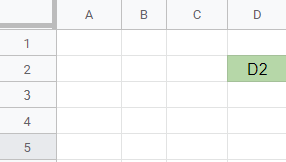
\includegraphics[width=1\linewidth]{C:/Users/rodri/OneDrive/Documentos/UFRGS/Disciplinas/estatistica_descritiva/MAT02018/images/planilha_eletro} \caption[Célula D2, no cruzamento da coluna D com a linha 2]{Célula D2, no cruzamento da coluna D com a linha 2.}\label{fig:fig-plan_eletro}
\end{marginfigure}

\textbf{Exemplo:} considere o exemplo adaptado de
\citep{morettin_estatistica_2017}. Um pesquisador está interessado em
fazer um levantamento sobre alguns aspectos socioeconômicos dos
empregados da seção de orçamentos da Companhia MB, um grupo de 15
pessoas. Temos a seguinte planilha (Fig. 2) para registrar os dados do
grupo.

\begin{figure}
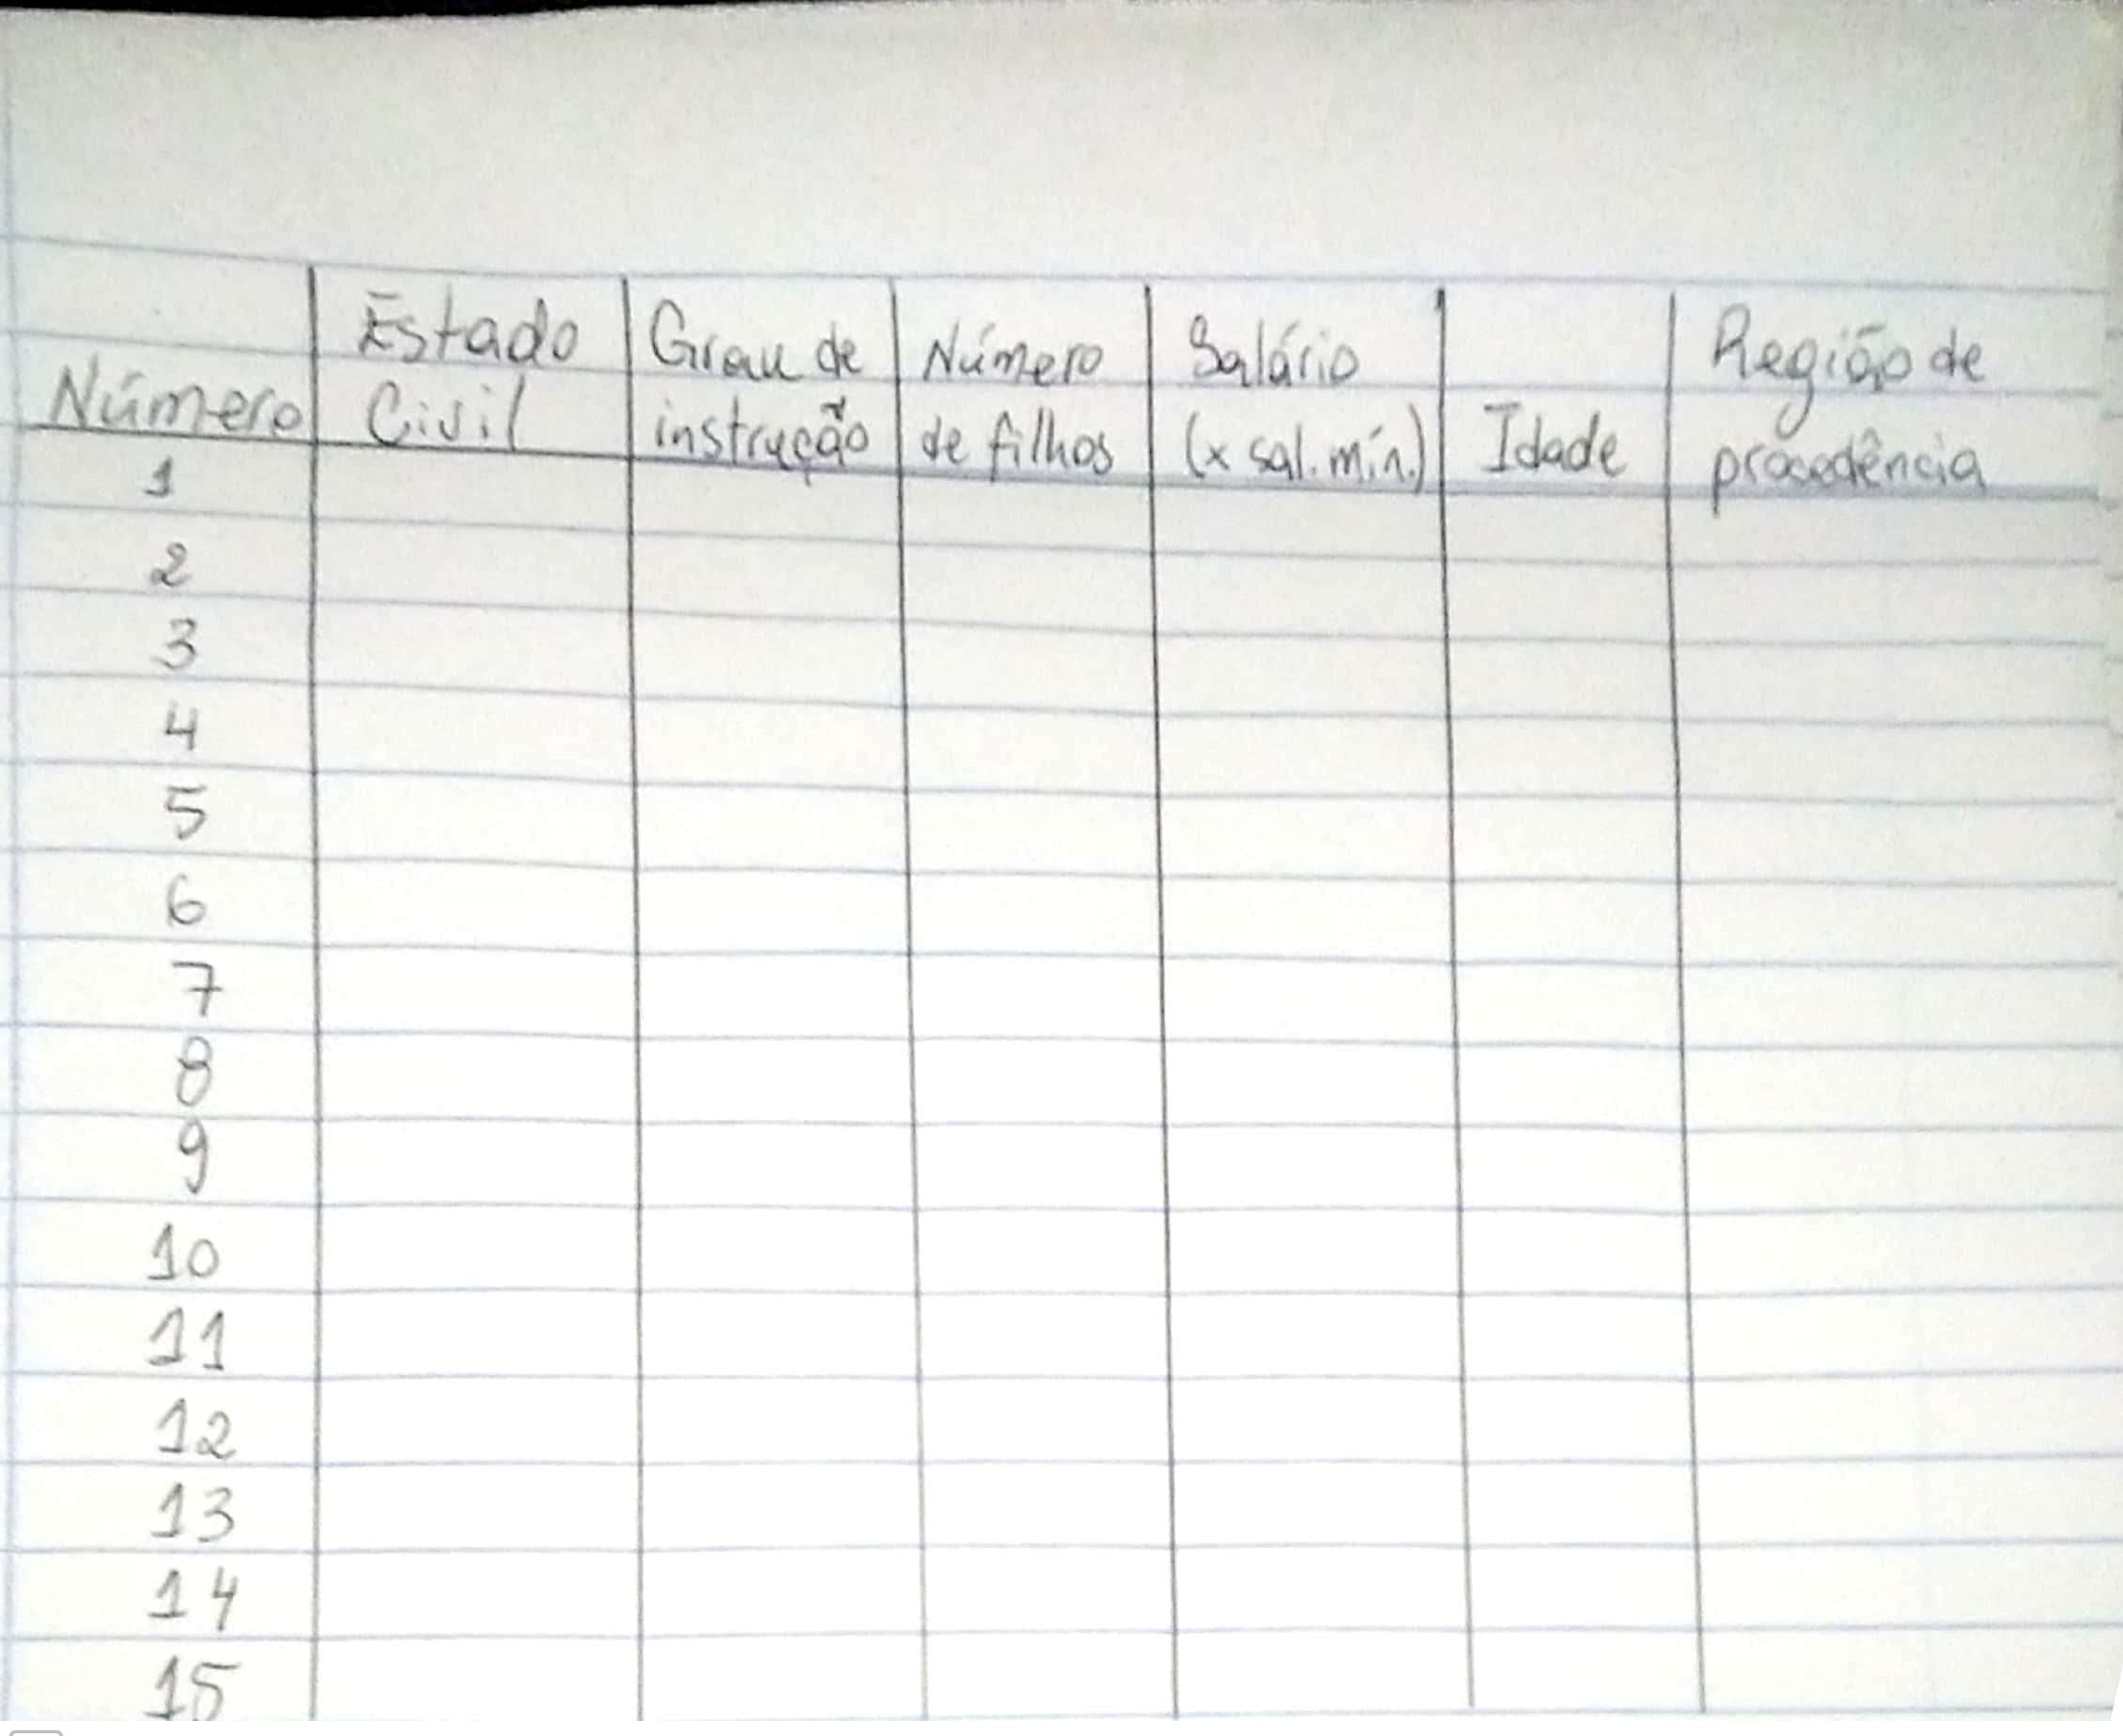
\includegraphics[width=1\linewidth]{C:/Users/rodri/OneDrive/Documentos/UFRGS/Disciplinas/estatistica_descritiva/MAT02018/images/planilha_fisica} \caption[Planilha física para o registro dos dados do grupo de 15 empregados da seção de orçamentos da Companhia MB]{Planilha física para o registro dos dados do grupo de 15 empregados da seção de orçamentos da Companhia MB.}\label{fig:fig-plan_fis}
\end{figure}

\begin{itemize}
\tightlist
\item
  \textbf{Dados brutos} são os dados na forma em que foram coletados,
  sem qualquer tipo de tratamento.
\end{itemize}

Após a coleta de dados, o pesquisador tem em sua planilha o registro dos
dados brutos (Fig. 3).

\begin{figure}
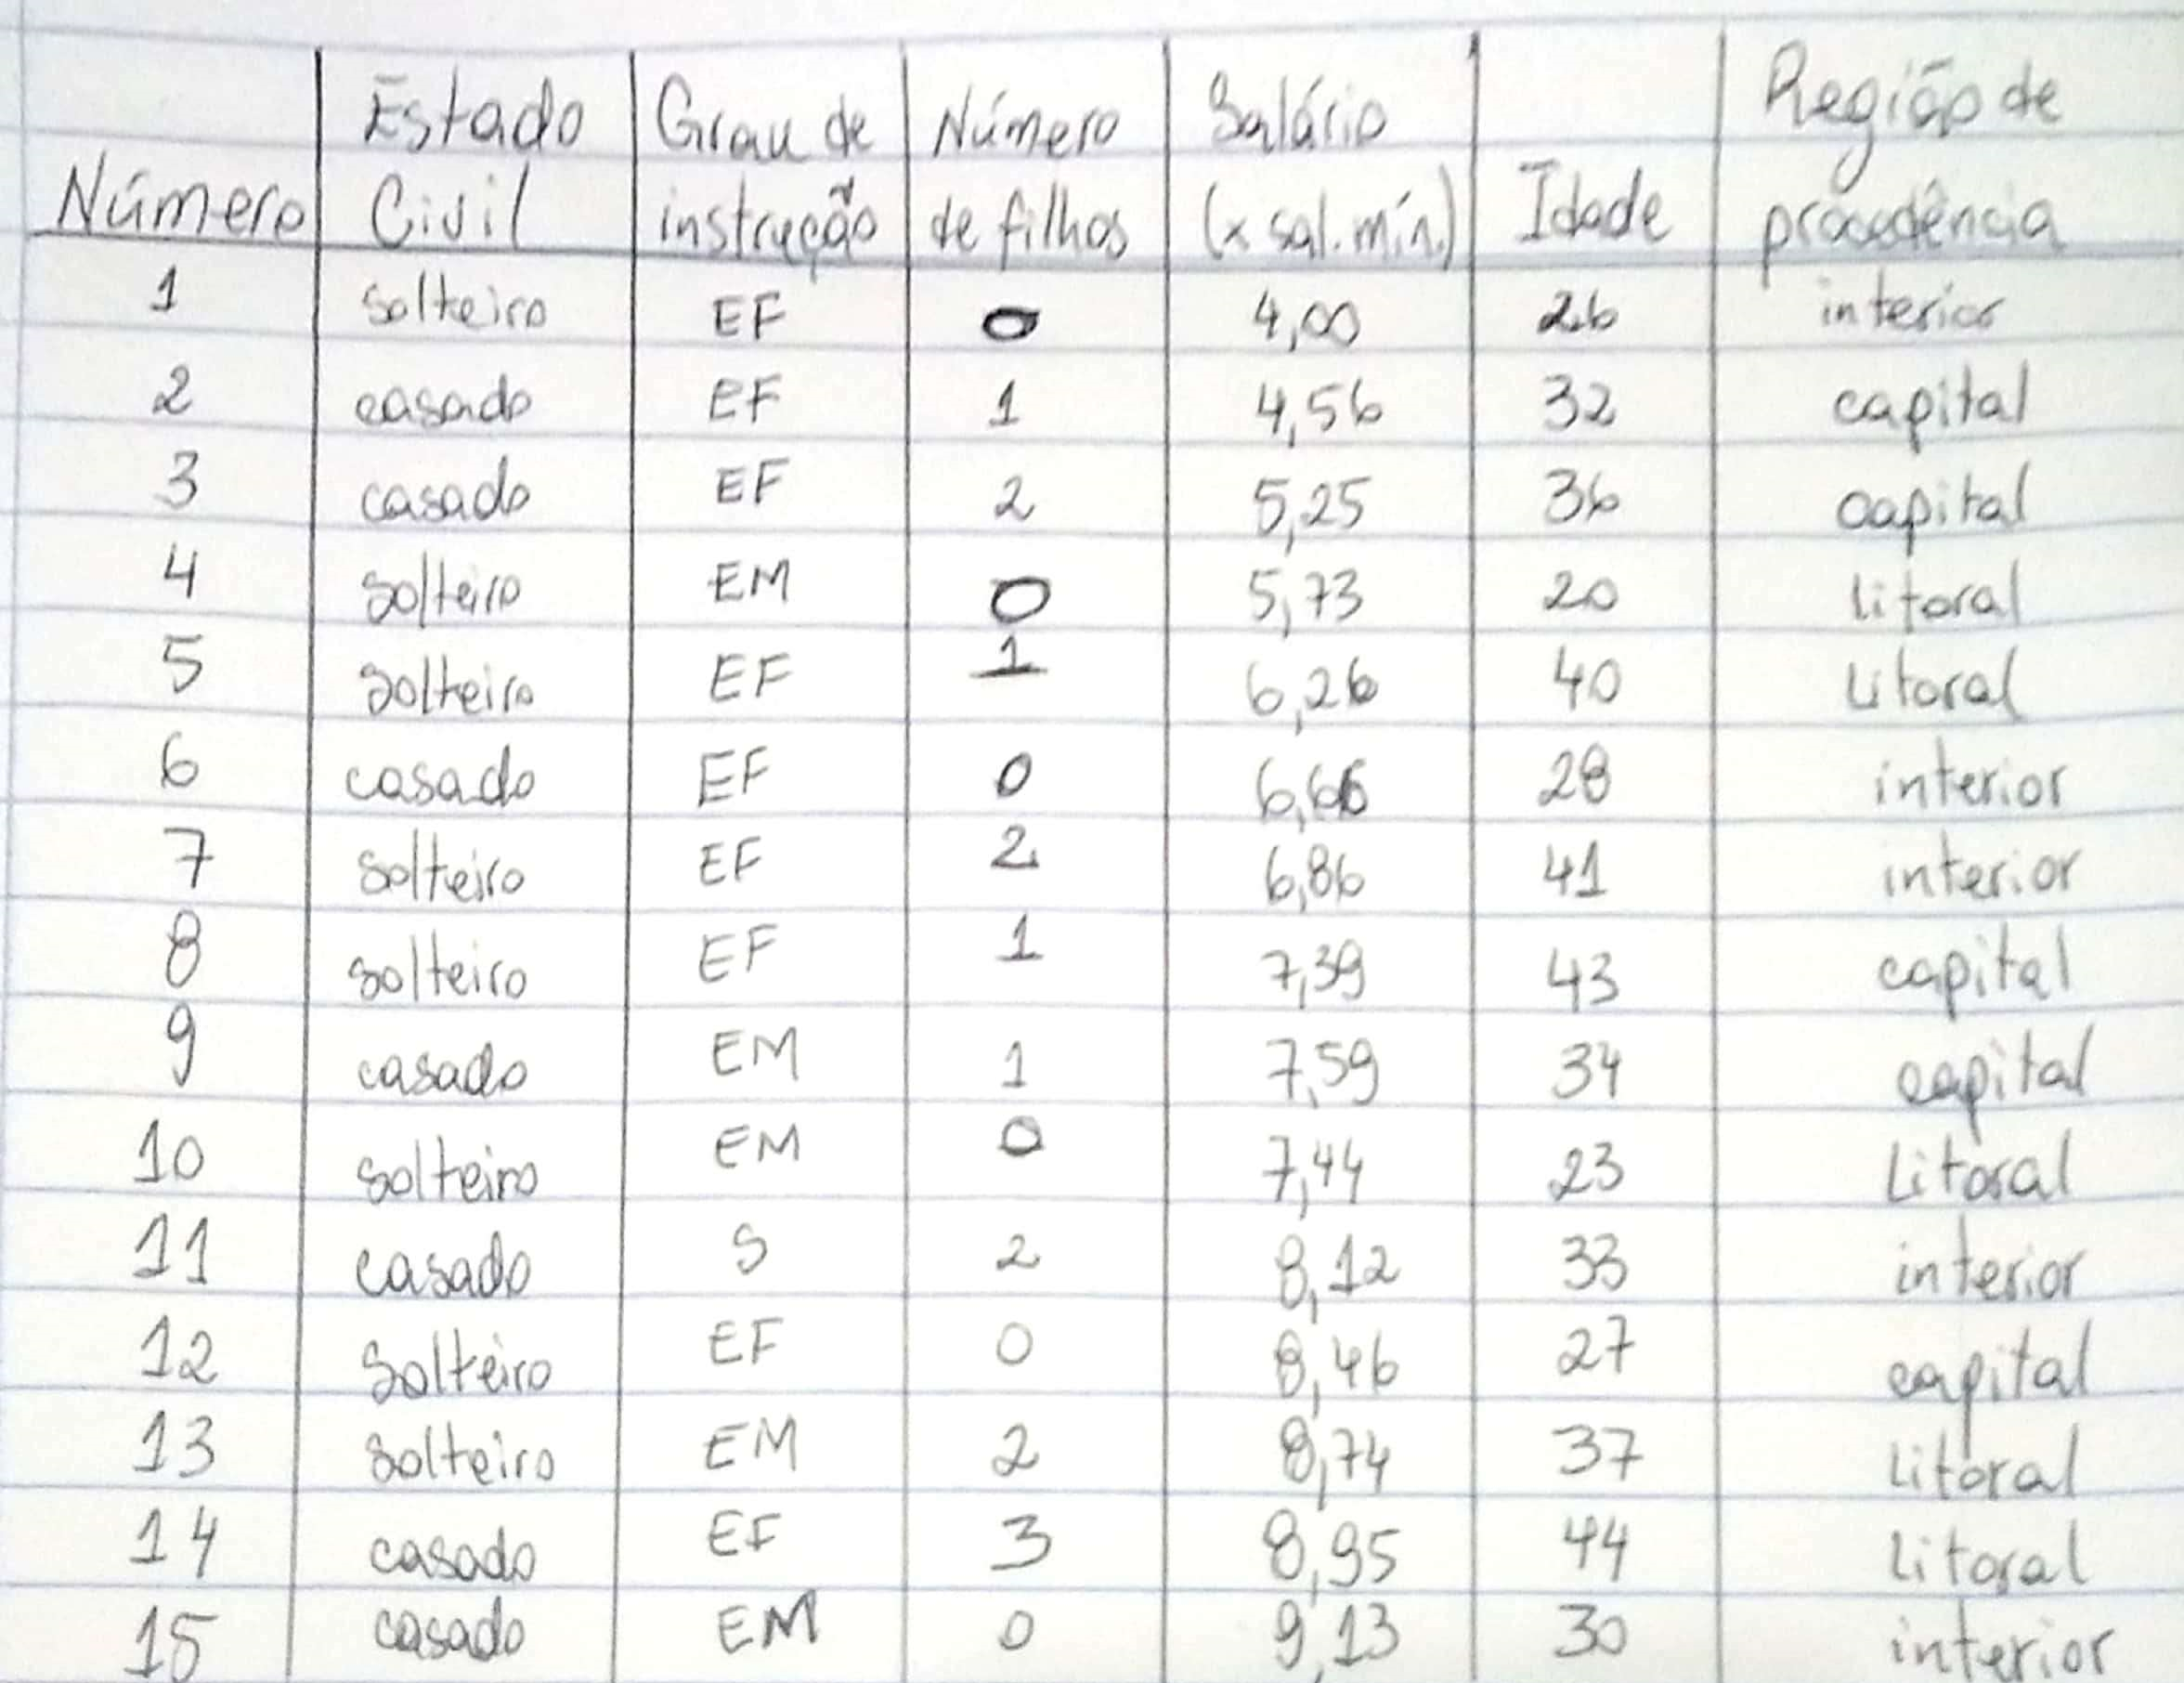
\includegraphics[width=1\linewidth]{C:/Users/rodri/OneDrive/Documentos/UFRGS/Disciplinas/estatistica_descritiva/MAT02018/images/dados_brutos} \caption[Planilha com o registro dos dados brutos do grupo de 15 empregados da seção de orçamentos da Companhia MB]{Planilha com o registro dos dados brutos do grupo de 15 empregados da seção de orçamentos da Companhia MB. EF, EM e S representam Ensino Fundamental, Ensino Médio e Superior, respectivamente.}\label{fig:fig-dados_brutos}
\end{figure}

\begin{itemize}
\tightlist
\item
  O que podemos falar sobre as variáveis coletadas?
\item
  Qual a informação podemos apresentar sobre os dados coletados?
\end{itemize}

Para responder tais perguntadas, precisaremos \textbf{resumir} os dados
de alguma forma. Na próxima seção discutiremos a etapa de
\textbf{apuração dos dados}.

\begin{itemize}
\tightlist
\item
  \textbf{Exercício:} construa a planilha para o registro do
  levantamento dos dados planejado nas aulas anteriores.
\end{itemize}

\hypertarget{apurauxe7uxe3o-dos-dados}{%
\section{Apuração dos dados}\label{apurauxe7uxe3o-dos-dados}}

\begin{itemize}
\tightlist
\item
  \textbf{Apuração} é o processo de retirar os dados da planilha e
  organizá-los, para apresentação.
\end{itemize}

No exemplo apresentado anteriormente, foram coletadas as seguintes
variáveis: estado civil, grau de instrução, número de filhos, salário,
idade e região de procedência. Note que estas são variáveis de
diferentes tipos\footnote{\textbf{Exercício:} classifique cada uma
  destas variáveis em \emph{qualitativa nominal}, \emph{qualitativa
  ordinal}, \emph{quantitativa discreta} e \emph{quantitativa contínua}.}.

\hypertarget{apurauxe7uxe3o-de-dados-nominais}{%
\subsection{Apuração de dados
nominais}\label{apurauxe7uxe3o-de-dados-nominais}}

Se quisermos saber quantos solteiros e quantos casados trabalham na
seção de orçamentos da Companhia MB devemos escrever os valores
possíveis da variável \emph{estado civil}\footnote{\textbf{Pergunta:} a
  ordem de escrita dos valores possíveis da variável \emph{estado civil}
  importa? Por que?}.

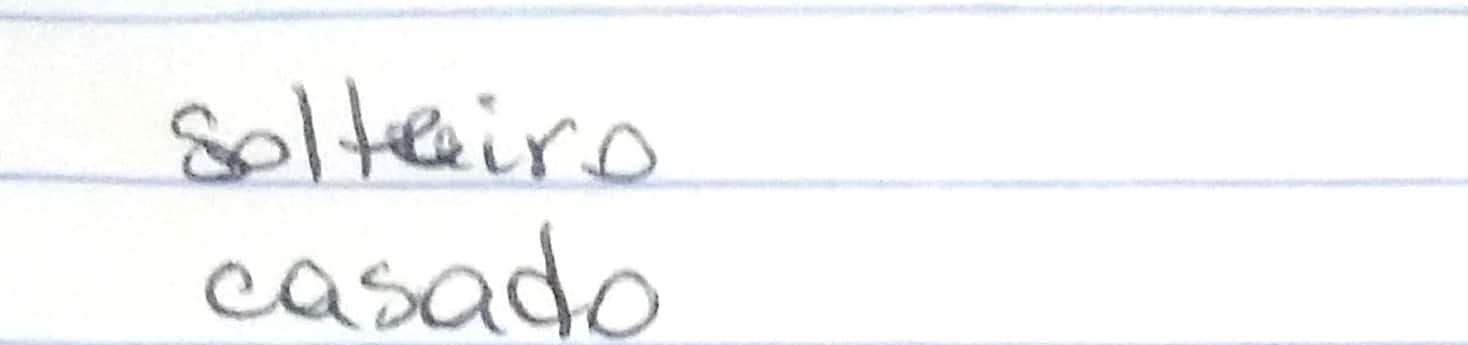
\includegraphics[width=0.7\linewidth]{C:/Users/rodri/OneDrive/Documentos/UFRGS/Disciplinas/estatistica_descritiva/MAT02018/images/apura_0}

Logo após, precisamos inspecionar cada registro da tabela de dados
brutos e marcar um traço ao lado de \emph{solteiro}, para cada indivíduo
solteiro inspecionado, e um traço ao lado de \emph{casado} para cada
indivíduo casado inspecionado. A cada quatro traços, corta-se com um
traço, e este conjunto representa uma contagem de cinco indivíduos
\footnote{No inglês, \emph{tally marks} (marcas de registro).}.

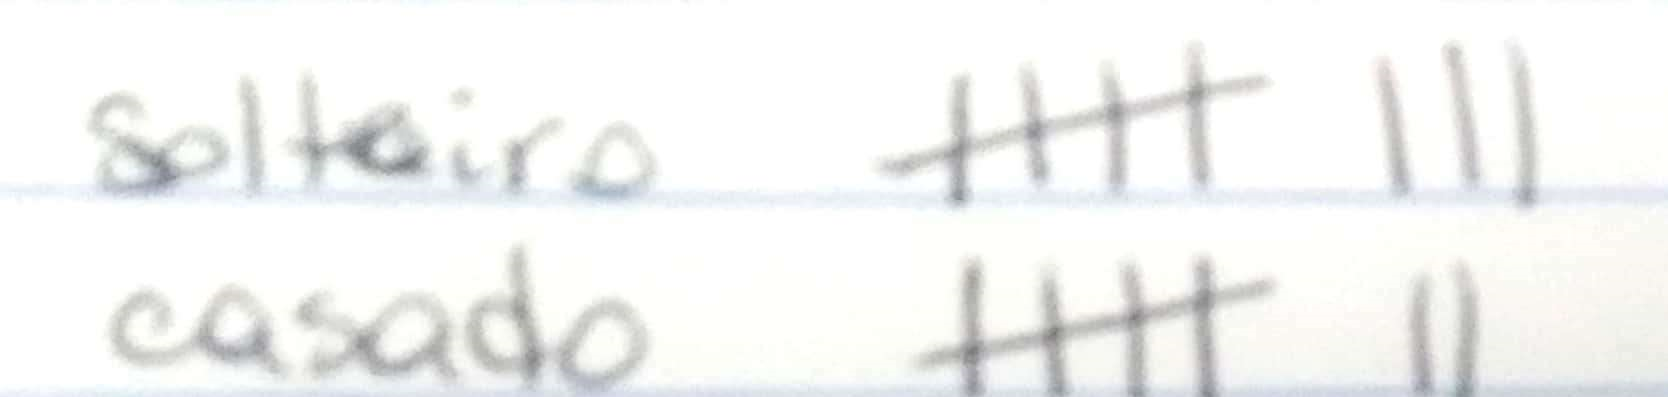
\includegraphics[width=0.7\linewidth]{C:/Users/rodri/OneDrive/Documentos/UFRGS/Disciplinas/estatistica_descritiva/MAT02018/images/apura_1}

Desta forma, verificamos que na seção de orçamentos da Companhia MB
trabalham oito solteiros e sete casados. Duas outras formas alternativas
de se fazer a apuração dos dados são apresentadas a seguir\footnote{\textbf{Comentário:}
  é fácil apurar uma pequena massa de dados, como no caso do exemplo. Já
  uma grande massa de dados tornará a tarefa difícil e entediante. Além
  disso, com um grande volume de dados, a \emph{probabilidade} de
  incorrermos em erros aumenta! Necessitaremos do auxílio de
  \emph{pacotes estatísticos}!}.

\begin{center}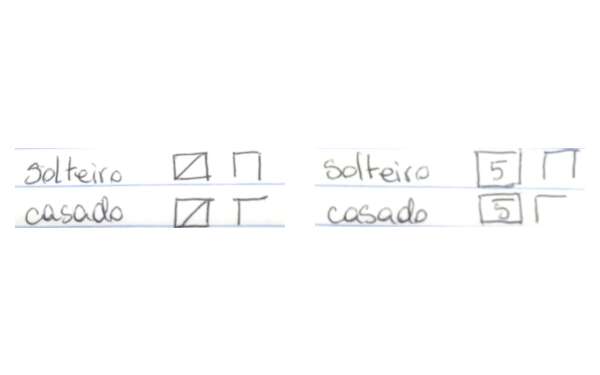
\includegraphics[width=1\linewidth]{organiza_dados_tint_files/figure-latex/fig-apura_2-1} \end{center}

\hypertarget{apurauxe7uxe3o-de-dados-ordinais}{%
\subsection{Apuração de dados
ordinais}\label{apurauxe7uxe3o-de-dados-ordinais}}

Para apurar dados de grau de instrução (variável qualitativa ordinal), o
procedimento é similar ao adotado para apurar dados nominais. A
diferença é que, para dados ordinais, \textbf{impõe-se uma ordem}.
Contudo, a apuração se faz por contagem.

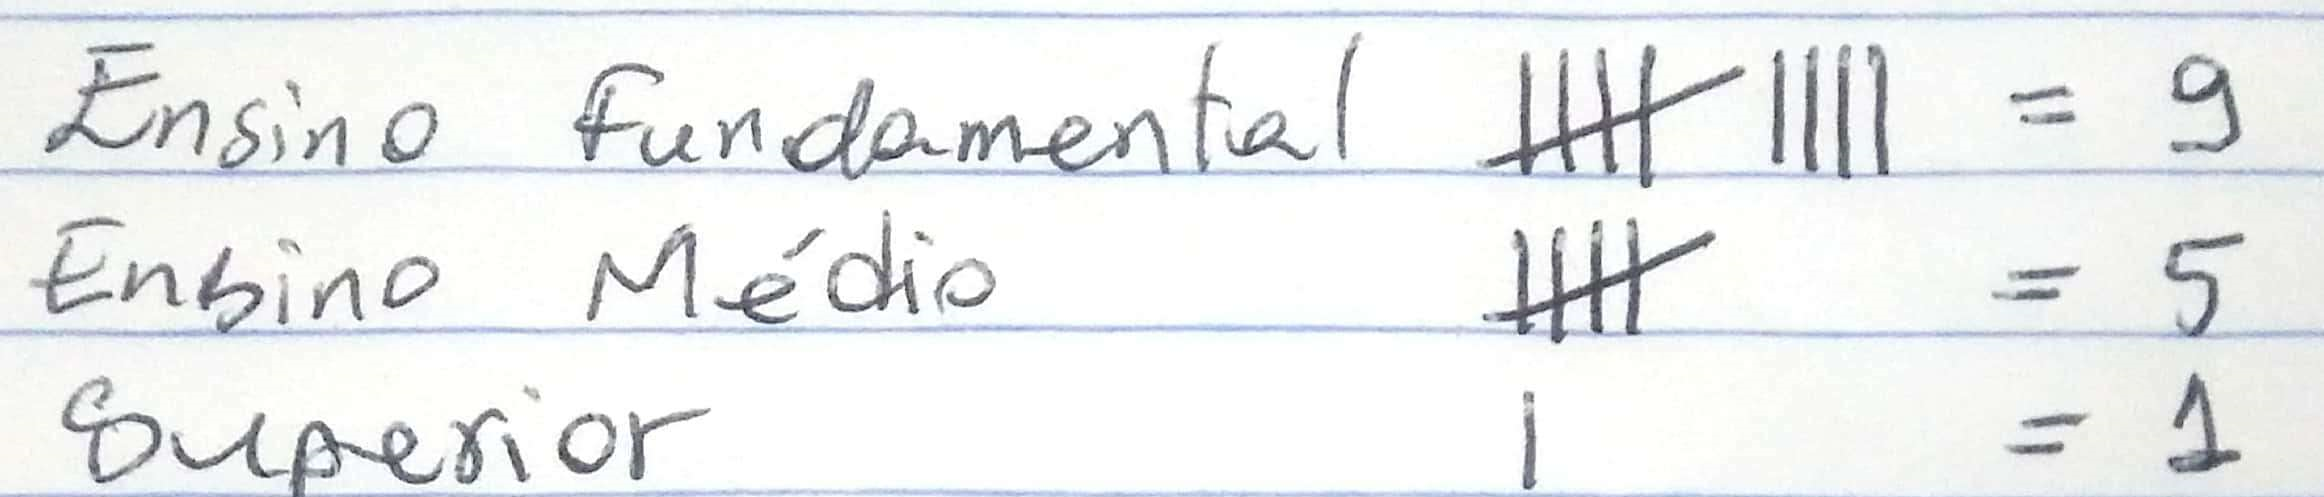
\includegraphics[width=0.7\linewidth]{C:/Users/rodri/OneDrive/Documentos/UFRGS/Disciplinas/estatistica_descritiva/MAT02018/images/apura_4}

\hypertarget{apurauxe7uxe3o-de-dados-discretos}{%
\subsection{Apuração de dados
discretos}\label{apurauxe7uxe3o-de-dados-discretos}}

Para apurar o número de filhos (variável quantitativa discreta), também
devemos fazer uma contagem. Escrevemos os resultados respeitando a ordem
numérica.

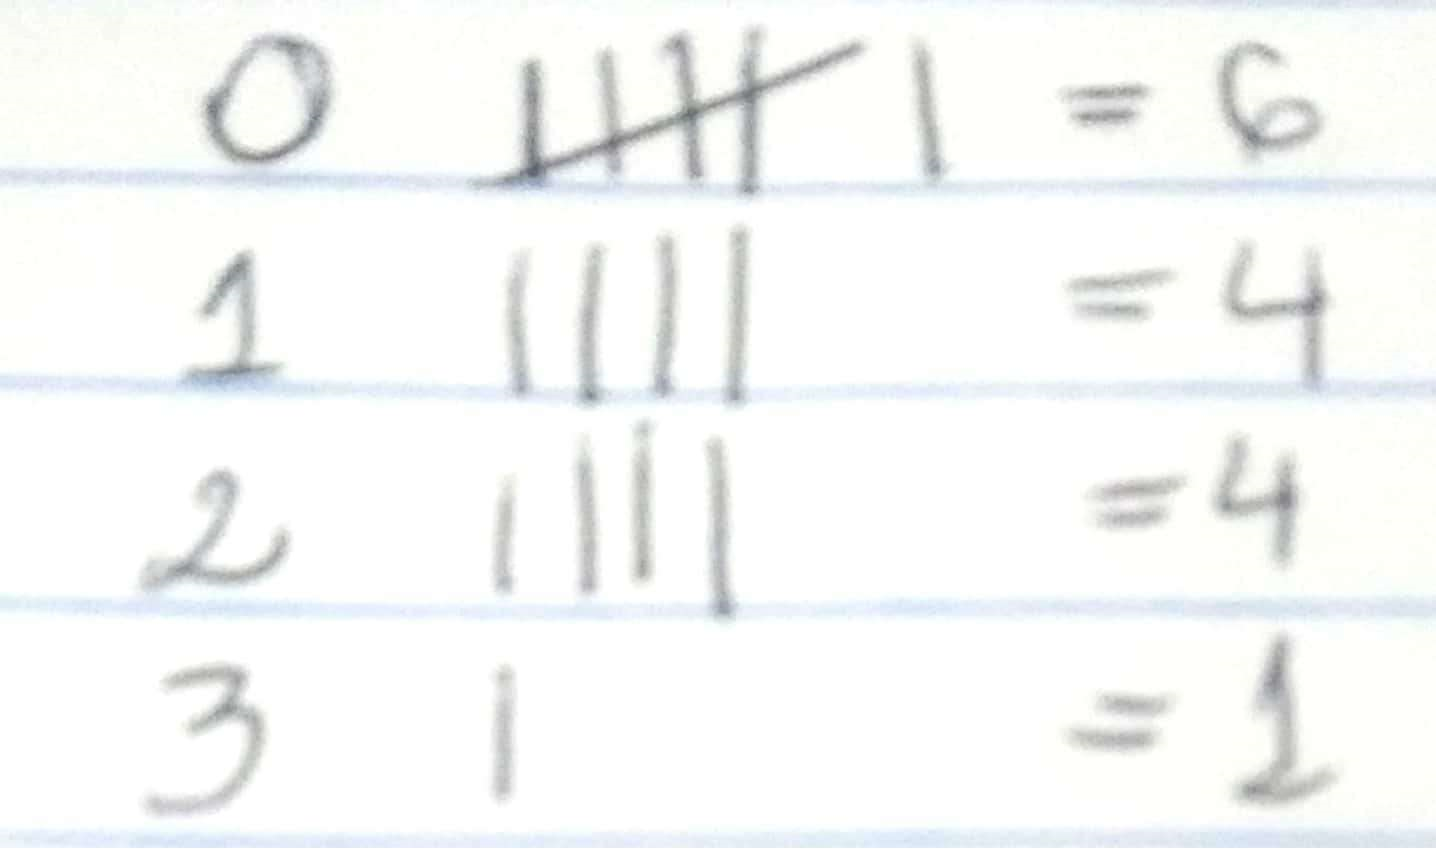
\includegraphics[width=0.7\linewidth]{C:/Users/rodri/OneDrive/Documentos/UFRGS/Disciplinas/estatistica_descritiva/MAT02018/images/apura_5}

\hypertarget{apurauxe7uxe3o-de-dados-contuxednuos}{%
\subsection{Apuração de dados
contínuos}\label{apurauxe7uxe3o-de-dados-contuxednuos}}

Em geral, os dados contínuos são apresentados na forma como foram
coletados, porque assumem valores diferentes, mesmo em amostras
pequenas. É o caso da variável idade no exemplo considerado: os
empregados da seção de orçamentos da Companhia MB tinham idades
diferentes. No entanto, é possível organizar as idades por faixas, como
veremos nas aulas seguintes.

\hypertarget{exercuxedcios}{%
\section{Exercícios}\label{exercuxedcios}}

Faça uma pequena coleta de dados incluindo pelo menos uma variável de
cada tipo (\emph{qualitativa nominal}, \emph{qualitativa ordinal},
\emph{quantitativa discreta} e \emph{quantitativa contínua}).

\begin{enumerate}
\def\labelenumi{\arabic{enumi}.}
\tightlist
\item
  Organize uma planilha (física ou eletrônica) para o registro dos dados
  coletados.
\item
  Faça a coleta e preencha a planilha para obter os dados brutos.
\item
  Faça a apuração dos dados e comente brevemente sobre os resultados
  encontrados.
\end{enumerate}

\hypertarget{complementar}{%
\section{\texorpdfstring{Complementa\texttt{R}}{ComplementaR}}\label{complementar}}

Esta seção é complementar. São apresentadas algumas poucas funções em
\texttt{R} relacionadas a discussão da aula. Para tal, vamos utilizar o
exemplo original de \citep{morettin_estatistica_2017} sobre os dados dos
empregados da seção de orçamentos da Companhia MB. A planilha eletrônica
correspondente encontra-se no arquivo \texttt{companhia\_mb.xlsx}. Vamos
começar carregando os dados para o \texttt{R}. Existem várias formas de
se carregar \textbf{arquivos de dados} em diferentes no \texttt{R}. Como
arquivo de interesse encontra-se no formato do Excel (xlsx), vamos
utilizar a função \texttt{read\_excel} do pacote
\texttt{readxl}\footnote{Caso você não tenha o pacote,
  instale-o:\texttt{install.packages("readxl")}.}.

\begin{Shaded}
\begin{Highlighting}[]
\CommentTok{# install.packages("readxl")}
\KeywordTok{library}\NormalTok{(readxl)}

\NormalTok{dados <-}\StringTok{ }\KeywordTok{read_excel}\NormalTok{(}\DataTypeTok{path =} \StringTok{"companhia_mb.xlsx"}\NormalTok{)}
\end{Highlighting}
\end{Shaded}

\begin{Shaded}
\begin{Highlighting}[]
\KeywordTok{class}\NormalTok{(dados) }\CommentTok{# classe do objeto dados}
\end{Highlighting}
\end{Shaded}

\begin{verbatim}
## [1] "tbl_df"     "tbl"        "data.frame"
\end{verbatim}

\begin{Shaded}
\begin{Highlighting}[]
\KeywordTok{dim}\NormalTok{(dados) }\CommentTok{# dimensão do objeto dados}
\end{Highlighting}
\end{Shaded}

\begin{verbatim}
## [1] 36  7
\end{verbatim}

Note que o objeto \texttt{dados} é uma tabela de dados bruto.

\begin{Shaded}
\begin{Highlighting}[]
\KeywordTok{head}\NormalTok{(dados) }\CommentTok{# apresenta as primeiras linhas do objeto dados}
\end{Highlighting}
\end{Shaded}

\begin{verbatim}
## # A tibble: 6 x 7
##       N `Estado Civil` `Grau de Instru~ `N de Filhos` `Salario (x Sal~ Idade
##   <dbl> <chr>          <chr>                    <dbl>            <dbl> <dbl>
## 1     1 solteiro       ensino fundamen~            NA             4       26
## 2     2 casado         ensino fundamen~             1             4.56    32
## 3     3 casado         ensino fundamen~             2             5.25    36
## 4     4 solteiro       ensino médio                NA             5.73    20
## 5     5 solteiro       ensino fundamen~            NA             6.26    40
## 6     6 casado         ensino fundamen~             0             6.66    28
## # ... with 1 more variable: `Região de Procedência` <chr>
\end{verbatim}

A função \texttt{table} retorna contagens dos valores de cada variável,
e portanto, podemos utilizar esta função para a apuração dos dados.

\begin{Shaded}
\begin{Highlighting}[]
\KeywordTok{table}\NormalTok{(dados}\OperatorTok{$}\StringTok{`}\DataTypeTok{Estado Civil}\StringTok{`}\NormalTok{) }\CommentTok{# apura dados nominais}
\end{Highlighting}
\end{Shaded}

\begin{verbatim}
## 
##   casado solteiro 
##       20       16
\end{verbatim}

\begin{Shaded}
\begin{Highlighting}[]
\KeywordTok{table}\NormalTok{(dados}\OperatorTok{$}\StringTok{`}\DataTypeTok{Grau de Instrução}\StringTok{`}\NormalTok{) }\CommentTok{# apura dados ordinais}
\end{Highlighting}
\end{Shaded}

\begin{verbatim}
## 
## ensino fundamental       ensino médio           superior 
##                 12                 18                  6
\end{verbatim}

\begin{Shaded}
\begin{Highlighting}[]
\KeywordTok{table}\NormalTok{(dados}\OperatorTok{$}\StringTok{`}\DataTypeTok{N de Filhos}\StringTok{`}\NormalTok{) }\CommentTok{# apura dados discretos}
\end{Highlighting}
\end{Shaded}

\begin{verbatim}
## 
## 0 1 2 3 5 
## 4 5 7 3 1
\end{verbatim}

\begin{Shaded}
\begin{Highlighting}[]
\NormalTok{dados}\OperatorTok{$}\NormalTok{Idade }\CommentTok{# apura dados contínuos}
\end{Highlighting}
\end{Shaded}

\begin{verbatim}
##  [1] 26 32 36 20 40 28 41 43 34 23 33 27 37 44 30 38 31 39 25 37 30 34 41 26 32
## [26] 35 46 29 40 35 31 36 43 33 48 42
\end{verbatim}

\bibliography{estatistica-descritiva.bib}



\end{document}
